%!TEX root = ./seminar.tex
\section{Smartphones as Digital Healthcare Devices}
While healthcare costs climb by the billions, smartphone users do as well as can be seen in Figure~\ref{fig:graphical_statistics_of_smartphone_users}. Their size and computational power serve as assistants for day to day activities and load off for the human brain \cite{barr2015brain}. From waking us up in the morning to social media being the last thing we close before we do the same to our eyes.
\begin{figure}[htpb]
    \centering
    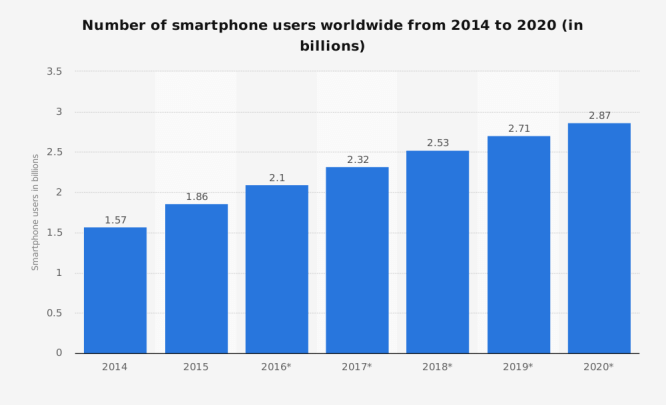
\includegraphics[width=0.8\linewidth]{media/Graphical-statistics-of-smartphone-users.png}
    \caption{Smartphone users worldwide \cite{numSmartphones}}%
    \label{fig:graphical_statistics_of_smartphone_users}
\end{figure}
\label{sec:smartphoneChances}
\subsection{Trackers}
Having these portable and computationally powerful devices everywhere we go, allows monitoring of various events throughout the day. In the last couple of years fitness tracker are on the rise, replacing traditional watches on peoples' wrists. Equipped with rechargeable batteries that last up to several months, processors that manage the various sensors and Bluetooth low energy technology to communicate data to a smartphone \cite{trackerDef}. The standard functionality of even the cheapest models include a heart rate monitor, step counter and of course a clock. This seemingly simple collection of data turned out to be of immense value in a case study from 2016 where a 42-year-old man was presented to the emergency department with newly diagnosed atrial fibrillation and otherwise normal physical examination. By looking at the synchronized data on his smartphone provided by his wrist-worn activity tracker, the medical staff was able to identify the onset of the arrhythmia as within the previous 3 hours, permitting eloctrocardioversion which is only applicable if the onset was less than 48 hours ago. The single correction of cardiovascular activity left the patient with a normal sinus rhythm at his follow-up appointment \cite{rudner2016interrogation}. \\
Another variety of trackers that is now just emerging includes monitoring of blood glucose levels. This allows diabetics to evaluate their blood glucose with the swipe of a finger and without the need to draw blood at all \cite{glucoseTracker}.
\subsection{Immediate Feedback}
The ability to monitor ones own health markers, as well as activities and react to them immediately, is a huge and time saving advantage over traditional healthcare environments where you either need to visit a doctor or have personal equipment like blood pressure or blood glucose measurement kits to get information about your current state of well being. Especially with the rise of chronic conditions and their quickly accumulating costs for patients and the healthcare system we saw earlier, this allows doctors to spend more time treating with more urgent matters and patients to enjoy life more with the time they save. Talking about enjoyment, it has been reported that people actively use the information provided by their health trackers to improve their current state of well being. Whether this includes getting into motion by trying to complete a daily step goal \cite{rasche2015activity} or calming themselves by observing an elevated heart rate, induced by stress \cite{mayya2015continuous}.
\subsection{The Future of Mobile Healthcare}
The industry around wearables has become gigantic during the last couple of year \cite{wearableMarket} and as the products become better and better, other aspects are far from perfect.
While activity trackers are great for providing data for smartphone apps to work with, the apps themselves play a significant part in patients' health. From the user interface to the quality of algorithms and user interactions, there is a lot to consider for mobile healthcare providers. Something that stands out in the context of mobile healthcare, delivered by smartphones, is that people with disabilities are not very well represented with respect to chronic health conditions. "Their omission in mHealth could lead to further disparities.", according to Jones et al. \cite{jones2018mobile}. As people with disabilities have additional requirements for treatment of chronic conditions, this leaves the providers of mobile healthcare with difficulties bringing their services to these patients. \\
Another issue in the mobile health sector is the quality of apps providing mental health services. While there are plenty of them out there, this quantity does not equal quality \cite{torous2017needed}. As a society, we just recently came to accept that mental health is important for all of us and suffering from depression and other mental conditions is a serious matter \cite{bharadwaj2017mental}. With stigmas around the issue falling away, patients seek primarily trust and understanding of their condition. Many applications offer real-time capture of environmental context with smartphone sensors. This helps patients tracking progress over time and identify triggers for relapses among other things. Others try intervention strategies. What is missing, are applications that bridge the gap between both approaches. Attempts at this have been made \cite{torous2019creating}, but these are just now emerging.
